%!TEX TS-program = xelatex

\documentclass[t]{beamer}

\usetheme{Hannover}
\usecolortheme{rose}

\usepackage{fontspec,xltxtra,xunicode}      %% подготавливает загрузку шрифтов Open Type, True Type и др.
%\defaultfontfeatures{Ligatures={TeX},Renderer=Basic}  %% свойства шрифтов по умолчанию
\setmainfont[Ligatures={TeX,Historic},
SmallCapsFont={Brill},
SmallCapsFeatures={Letters=SmallCaps}]{Brill} %% задаёт основной шрифт документа
\setsansfont{Brill}                    %% задаёт шрифт без засечек
\setmonofont[Ligatures=NoCommon]{DejaVu Sans}
\newfontfamily\SYM{Brill}
\usepackage{indentfirst}
%%% Дополнительная работа с математикой
\usepackage{amsmath,amsfonts,amssymb,amsthm,mathtools} % AMS
\usepackage{icomma} % "Умная" запятая: $0,2$ --- число, $0, 2$ --- перечисление

%%% Работа с картинками
\usepackage{wrapfig} % Обтекание рисунков текстом
\usepackage{rotating}
\usepackage{fixltx2e}
\usepackage{hhline}
\usepackage{lscape}

%%% Работа с таблицами
\usepackage{array,tabularx,tabulary,booktabs} % Дополнительная работа с таблицами
\usepackage{longtable}  % Длинные таблицы
\usepackage{multirow} % Слияние строк в таблице

\usepackage{multicol} % Несколько колонок
%%% Страница
%\usepackage{fancyhdr} % Колонтитулы
% 	\pagestyle{fancy}
 	%\renewcommand{\headrulewidth}{0pt}  % Толщина линейки, отчеркивающей верхний колонтитул
% 	\lfoot{Нижний левый}
% 	\rfoot{Нижний правый}
% 	\rhead{Верхний правый}
% 	\chead{Верхний в центре}
% 	\lhead{Верхний левый}
%	\cfoot{Нижний в центре} % По умолчанию здесь номер страницы

\usepackage{setspace} % Интерлиньяж
%\onehalfspacing % Интерлиньяж 1.5
%\doublespacing % Интерлиньяж 2
\singlespacing % Интерлиньяж 1

\usepackage{subfig} % подкартинки
\usepackage{lastpage} % Узнать, сколько всего страниц в документе.
\usepackage{soul} % Модификаторы начертания
\usepackage{bbding}
\usepackage{tikz} % Работа с графикой
\usepackage{pgfplots}
\usepackage{pgfplotstable}
\usepackage{verbatim}

\usepackage{attachfile2}
\usepackage{alltt}

%%% Лингвистические пакеты
%\usepackage{savetrees} % пакет, который экономит место
\usepackage{forest} % для рисования деревьев
\usepackage{vowel} % для рисования трапеций гласных
\usepackage{natbib}
\bibpunct[: ]{[}{]}{;}{a}{}{,}
\usepackage[nogroupskip,nopostdot, nonumberlist]{glossaries}
%\usepackage{glossary-mcols} 
%\setglossarystyle{mcolindex}
\usepackage{philex} % пакет для примеров
\newcommand{\mytem}{\item[$\circ$]}
\addto\captionsrussian{
\renewcommand{\refname}{}}

\newcommand{\apostrophe}{\XeTeXglyph\XeTeXcharglyph"0027\relax}
\usetikzlibrary{patterns}

\usepackage{ulem}

\usepackage{hyperref}
\setbeamercolor{alerted text}{fg=blue}
\setbeamersize{text margin left=4mm,text margin right=1mm} 
\setbeamertemplate{frametitle}[default][center]
\setbeamertemplate{navigation symbols}{
	\usebeamerfont{footline}%
    \usebeamercolor[fg]{footline}%
    \hspace{1em}%
    {{\small презентация доступна: \href{https://tinyurl.com/y4fuuxt5}{\textbf{tinyurl.com/y4fuuxt5}}}
    \hspace{4cm}
    \insertframenumber/\inserttotalframenumber\vspace{0.5mm}}}
\title[]{Computer Speech technologies}
\author[]{G. Moroz}
\date{21 March, 2019}
\begin{document}
\frame{\titlepage}

\section{first attempts}

\begin{frame}{Wolfgang Ritter \href{https://books.google.ru/books?hl=pl&lr=&id=3MRJAAAAcAAJ&oi=fnd&pg=PA1&dq=Mechanismus+der+menschlichen+Sprache+nebst+Beschreibung+einer+sprechenden+Maschine&ots=MW2q1Xb0dG&sig=qwlXuPxE6P_Ruryv-FXckqV10Pk&redir_esc=y\#v=onepage&q=Mechanismus\%20der\%20menschlichen\%20Sprache\%20nebst\%20Beschreibung\%20einer\%20sprechenden\%20Maschine&f=false}{\cite[76]{kempelen91}}}
\centering
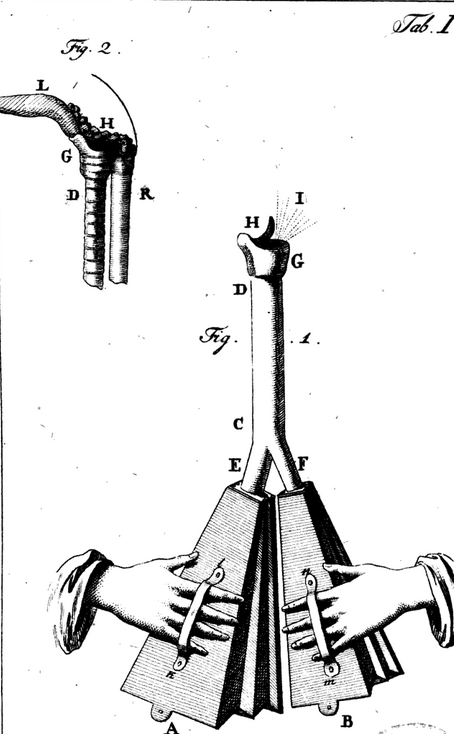
\includegraphics[width=0.45\linewidth]{01-kempelen}
\end{frame}

\begin{frame}{Wolfgang Ritter \href{https://books.google.ru/books?hl=pl&lr=&id=3MRJAAAAcAAJ&oi=fnd&pg=PA1&dq=Mechanismus+der+menschlichen+Sprache+nebst+Beschreibung+einer+sprechenden+Maschine&ots=MW2q1Xb0dG&sig=qwlXuPxE6P_Ruryv-FXckqV10Pk&redir_esc=y\#v=onepage&q=Mechanismus\%20der\%20menschlichen\%20Sprache\%20nebst\%20Beschreibung\%20einer\%20sprechenden\%20Maschine&f=false}{\cite[107]{kempelen91}}}
\centering
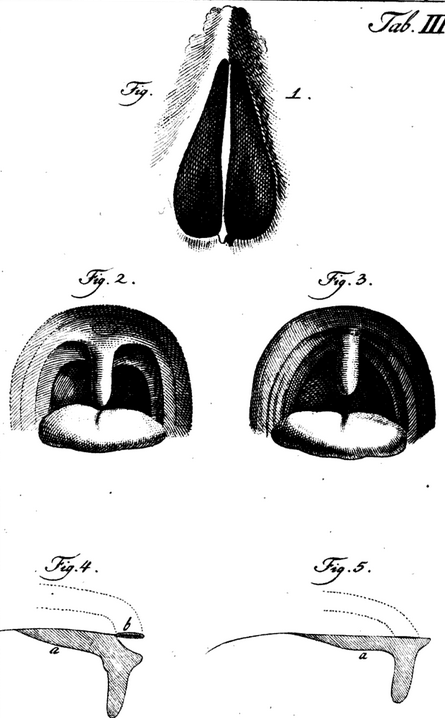
\includegraphics[width=0.45\linewidth]{02-kempelen}
\end{frame}

\begin{frame}{Wolfgang Ritter \href{https://books.google.ru/books?hl=pl&lr=&id=3MRJAAAAcAAJ&oi=fnd&pg=PA1&dq=Mechanismus+der+menschlichen+Sprache+nebst+Beschreibung+einer+sprechenden+Maschine&ots=MW2q1Xb0dG&sig=qwlXuPxE6P_Ruryv-FXckqV10Pk&redir_esc=y\#v=onepage&q=Mechanismus\%20der\%20menschlichen\%20Sprache\%20nebst\%20Beschreibung\%20einer\%20sprechenden\%20Maschine&f=false}{\cite[110]{kempelen91}}}
\centering
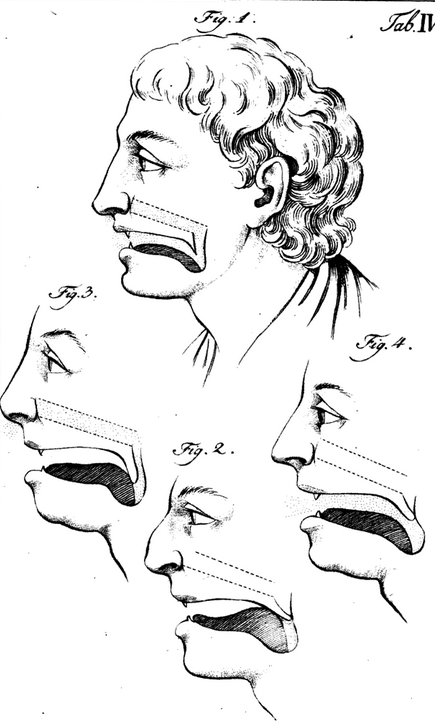
\includegraphics[width=0.45\linewidth]{03-kempelen}
\end{frame}

\begin{frame}{Wolfgang Ritter \href{https://books.google.ru/books?hl=pl&lr=&id=3MRJAAAAcAAJ&oi=fnd&pg=PA1&dq=Mechanismus+der+menschlichen+Sprache+nebst+Beschreibung+einer+sprechenden+Maschine&ots=MW2q1Xb0dG&sig=qwlXuPxE6P_Ruryv-FXckqV10Pk&redir_esc=y\#v=onepage&q=Mechanismus\%20der\%20menschlichen\%20Sprache\%20nebst\%20Beschreibung\%20einer\%20sprechenden\%20Maschine&f=false}{\cite[144]{kempelen91}}}
\centering
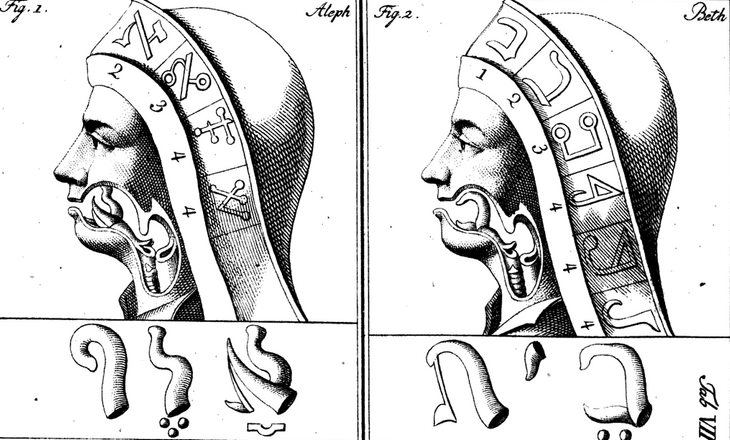
\includegraphics[width=\linewidth]{04-kempelen}
\end{frame}

\begin{frame}{W. R. von Kempelen: chess-playing ``automaton''}
\centering
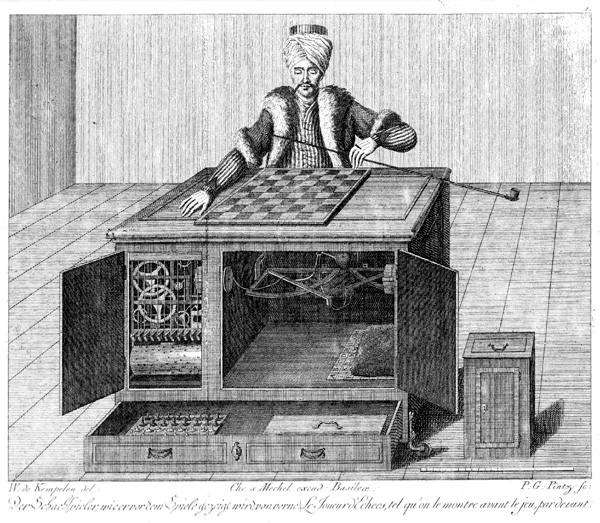
\includegraphics[width=0.85\linewidth]{05-kempelen}
\end{frame}

\begin{frame}{Development of vowel production theory}
\begin{itemize}
\item Christian Gottlieb von Kratzenstein
\item W. Willis
\item Sir Charles Wheatstone
\item Hermann von Helmholtz
\item L. Hermann
\item Alexander Melville Bell and Alexander Graham Bell
\end{itemize}
\end{frame}

\section{vocoder}
\begin{frame}{Vocoder}
\begin{itemize}
\item In 1928 Bell Labs engineer Homer Dudley invented vocoder. \href{https://archive.org/stream/bellsystemtechni19amerrich/bellsystemtechni19amerrich\#page/495/mode/1up}{\cite[508]{dudley40}}.
\end{itemize}
\centering
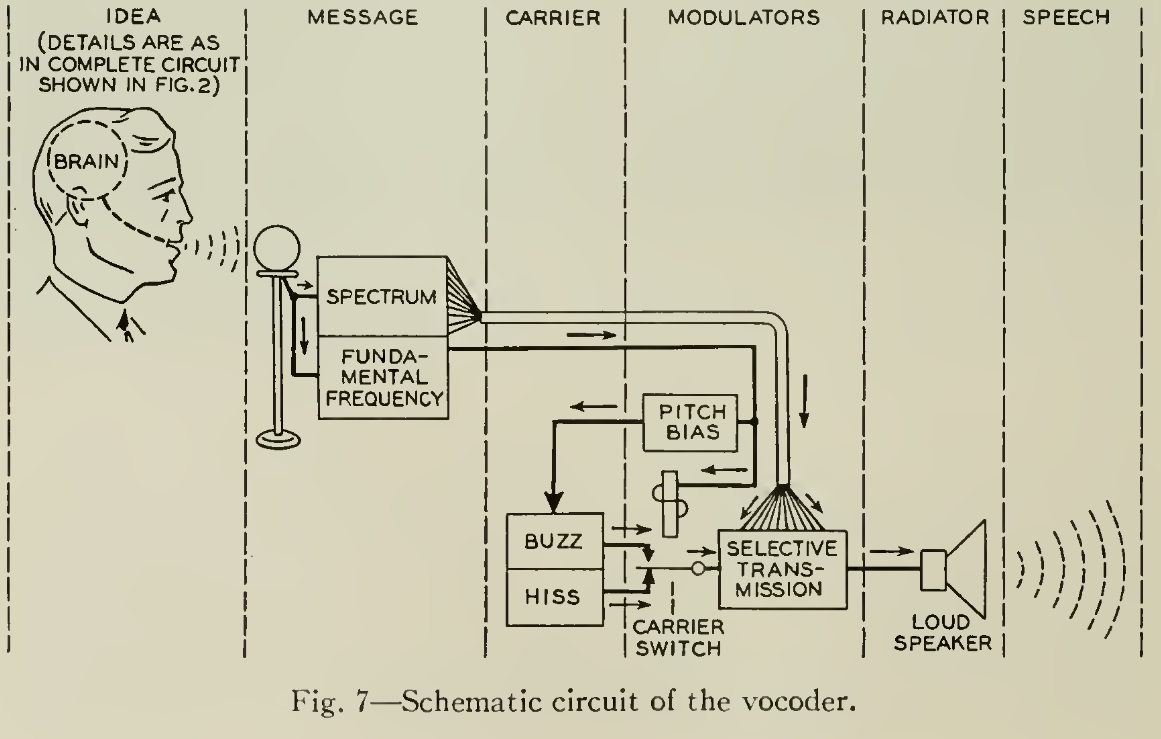
\includegraphics[width=\linewidth]{06-dudley}
\end{frame}

\section{vocoder}
\begin{frame}{Vocoder}
\begin{itemize}
\item In 1928 Bell Labs engineer Homer Dudley invented vocoder. \href{https://archive.org/stream/bellsystemtechni19amerrich/bellsystemtechni19amerrich\#page/495/mode/1up}{\cite[509]{dudley40}}.
\end{itemize}
\centering
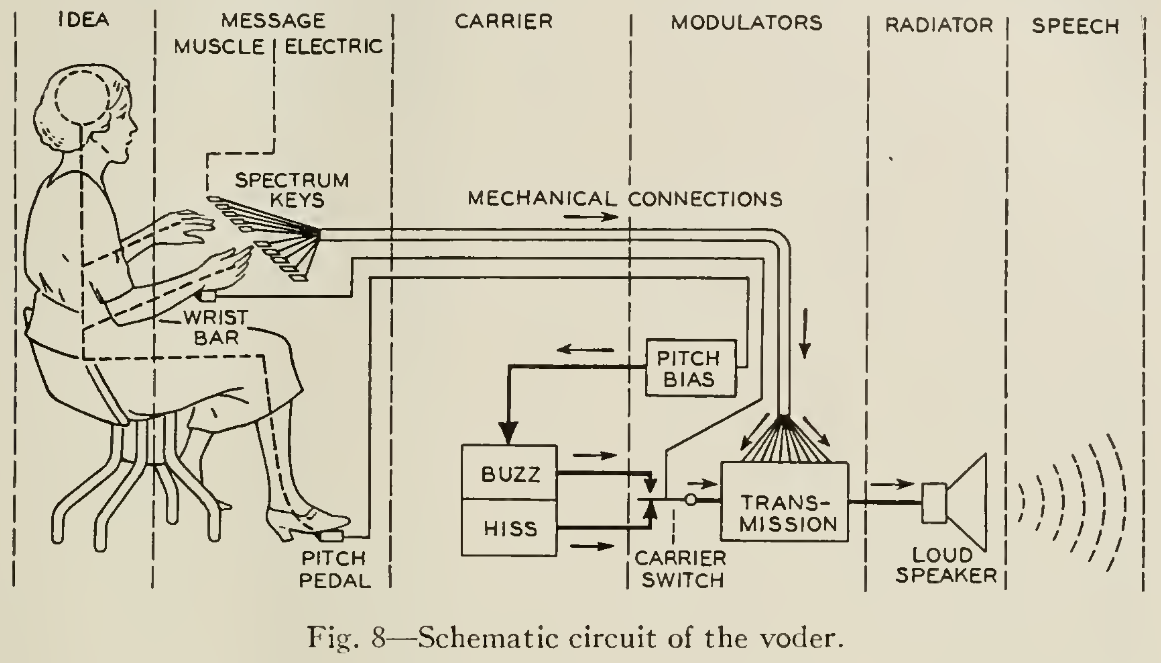
\includegraphics[width=\linewidth]{07-dudley}
\end{frame}

\section{important inventions}
\begin{frame}{Important inventions}
\begin{itemize}
\item Furier transform
\item Linear predicting coding (LPC)
\item Mel-frequency cepstrum (MFC)
\item \href{http://stevehanov.ca/wavelet/}{Wavelets}
\end{itemize}
\end{frame}

\begin{frame}{Wavelet: from Martti Vainio presentation 2017}
\vfill
\centering
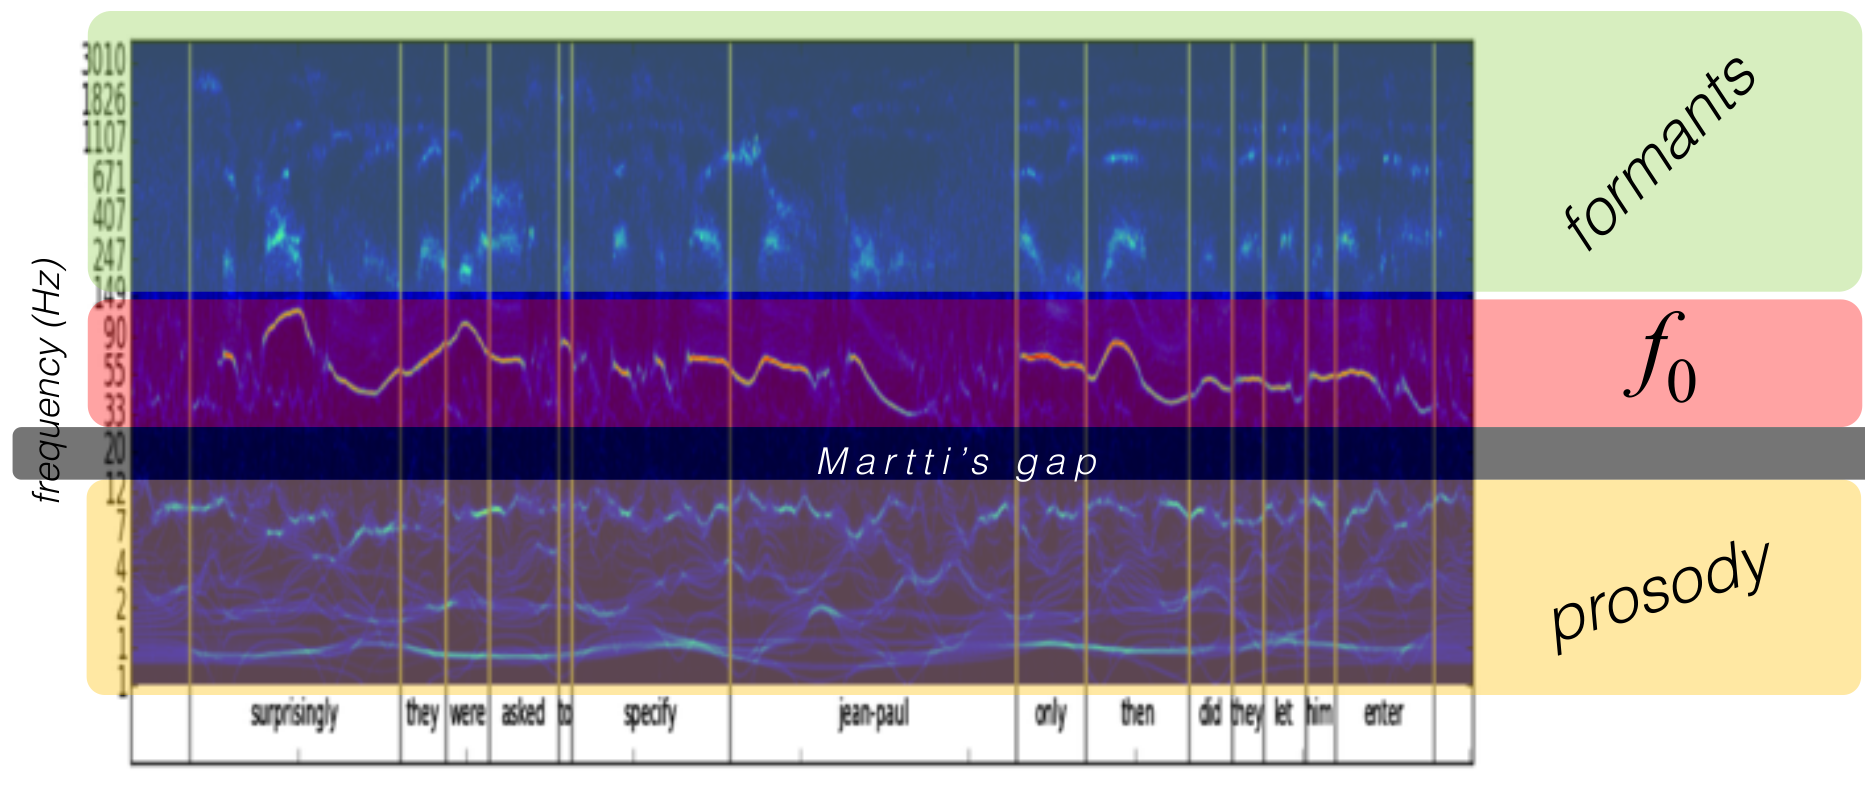
\includegraphics[width=\linewidth]{08-wavelet}
\end{frame}

\begin{frame}{Wavelet: from Martti Vainio presentation 2017}
\vfill
\centering
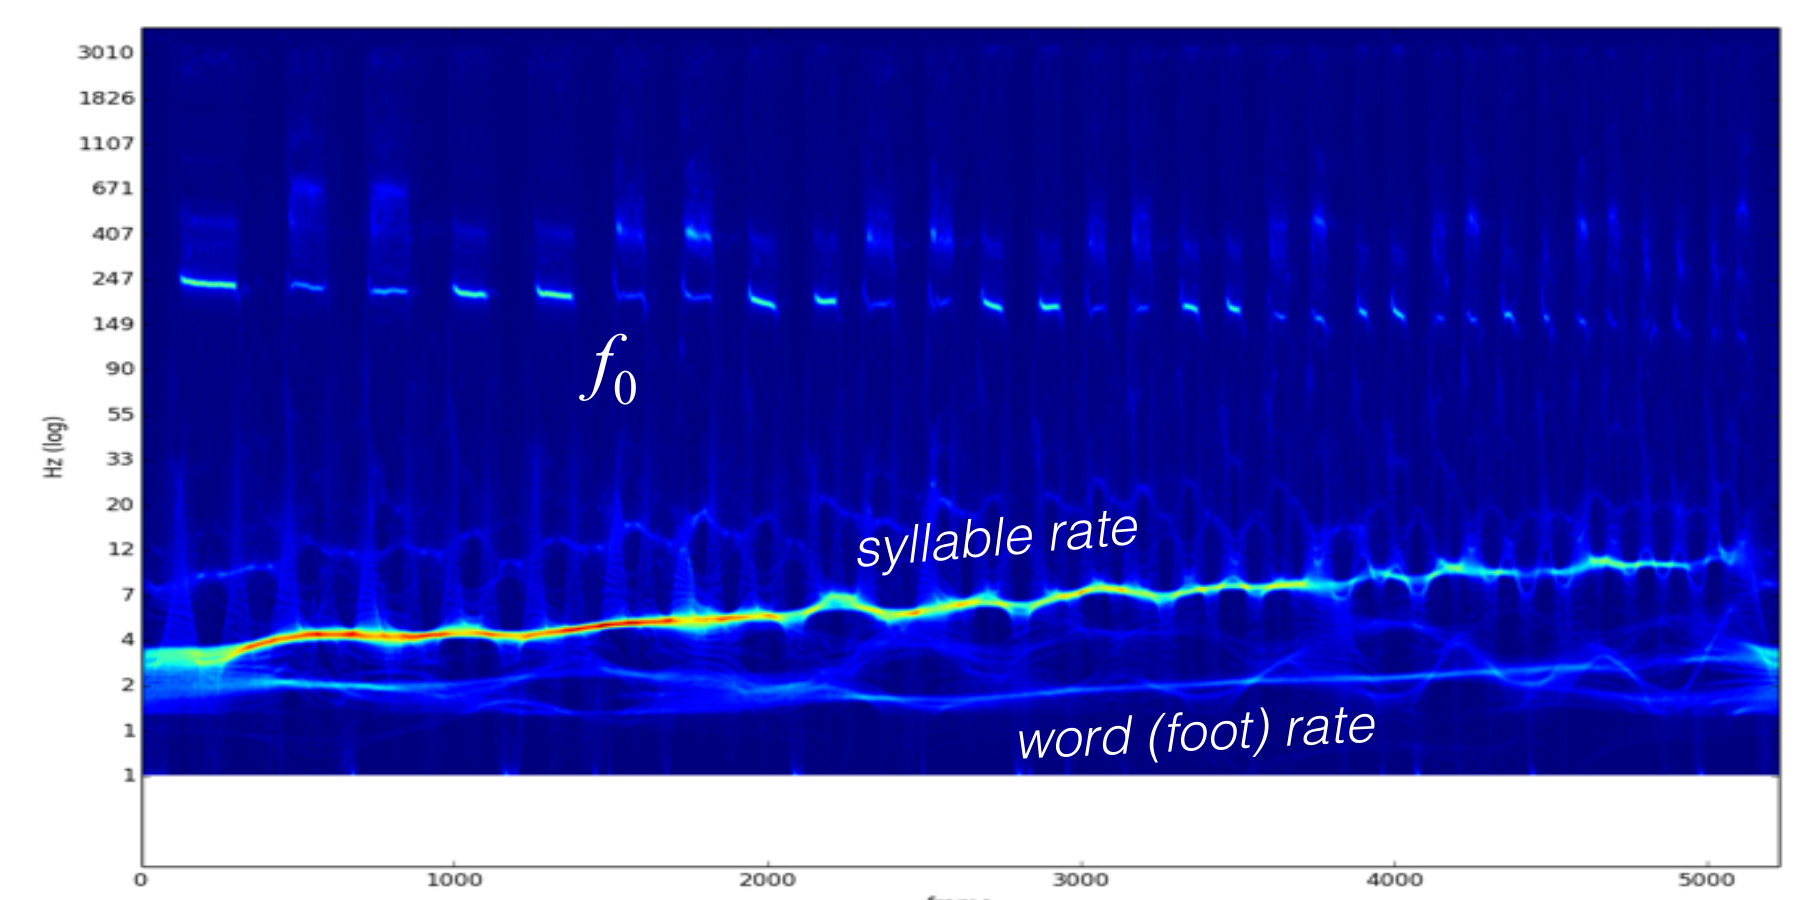
\includegraphics[width=\linewidth]{09-wavelet}
\end{frame}

\section{speech recognition}
\begin{frame}{Everybody dreams about speech recognition...}
\vfill
\pause
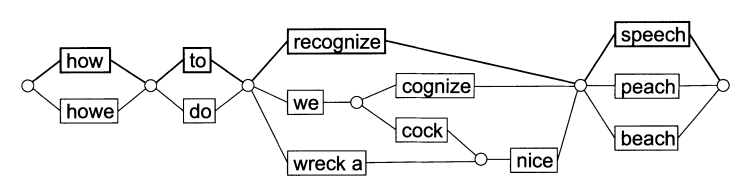
\includegraphics[width=\linewidth]{10-speech-recognition}
A word hypothesis graph returned by the speech recognition component for the utterance ``how to recognize speech''. \hfill after \cite[119]{schroeder13}
\end{frame}

\begin{frame}{Speech recognition}
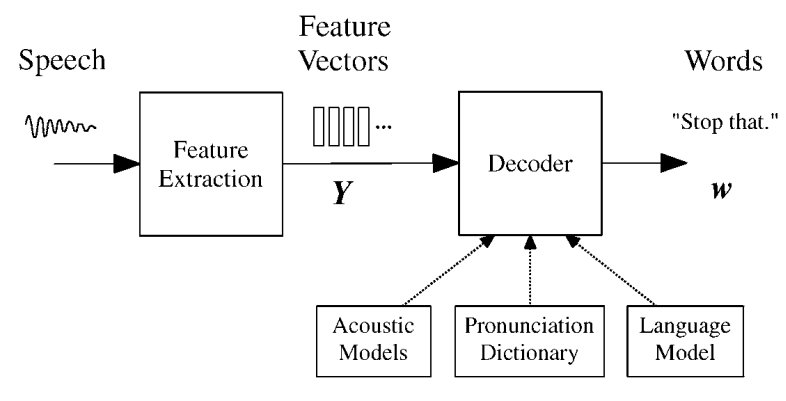
\includegraphics[width=0.95\linewidth]{11-speech-recognition}
after \cite[6]{gales07}\\

\begin{itemize}
\item Acoustic model: Hidden Markov Models or Deep Neural Network
\item Pronunciation dictionary: Decision tree, Markov Chain model, \textit{N}-gram language models
\item Language model: \textit{N}-gram models
\end{itemize}
\end{frame}

\section{other technologies}
\begin{frame}{Other Computer Speech technologies}
\begin{itemize}
\item Speech synthesis
\item Speaker Identification
\item Dialogue systems
\item Prosody dependent tasks
\end{itemize}
\end{frame}

\section{}
\begin{frame}
{\huge Thank you!\bigskip\\
\normalsize Please, don't hesitate to write me\\
agricolamz@gmail.com
\vspace{-130pt}}
\end{frame}
\begin{frame}{Reference}
\footnotesize
\bibliographystyle{chicago}
\bibliography{bibliography}
\end{frame}
\end{document}
